\section{Non-Portable Kernel-Based Programming Models}\label{sec:non-portable-kernel-based-programming-models}


\subsection{Fundamentals of GPU programming with CUDA and HIP}


\par
Unlike some cross-platform portability ecosystems, such as Alpaka, Kokkos, OpenCL, RAJA, and SYCL, which cater to multiple architectures, CUDA and HIP are solely focused on GPUs.
They provide extensive libraries, APIs, and compiler toolchains that optimize code execution on NVIDIA GPUs (in the case of CUDA) and both NVIDIA and AMD GPUs (in the case of HIP).
Because they are developed by the device producers, these programming models provide high-performance computing capabilities and offer advanced features like shared memory, thread synchronization, and memory management specific to GPU architectures.


\par
CUDA, developed by NVIDIA, has gained significant popularity and is widely used for GPU programming.
It offers a comprehensive ecosystem that includes not only the CUDA programming model but also a vast collection of GPU-accelerated libraries.
Developers can write CUDA kernels using C++ and seamlessly integrate them into their applications to harness the massive parallelism of GPUs.


\par
HIP, on the other hand, is an open-source project that aims to provide a more~\lq\lq portable\rq\rq~GPU programming interface.
It allows developers to write GPU code in a syntax similar to CUDA and provides a translation layer that enables the same code to run on both NVIDIA and AMD GPUs.
This approach minimizes the effort required to port CUDA code to different GPU architectures and provides flexibility for developers to target multiple platforms.


\par
By being closely tied to the GPU hardware, CUDA and HIP provide a level of performance optimization that may not be achievable with cross-platform portability ecosystems.
The libraries and toolchains offered by these programming models are specifically designed to exploit the capabilities of the underlying GPU architectures, enabling developers to achieve high performance.


\par
Developers utilizing CUDA or HIP can tap into an extensive ecosystem of GPU-accelerated libraries, covering various domains, including linear algebra, signal processing, image processing, machine learning, and more.
These libraries are highly optimized to take advantage of the parallelism and computational power offered by GPUs, allowing developers to accelerate their applications without having to implement complex algorithms from scratch.


\par
As mentioned before, CUDA and HIP are very similar so it makes sense to cover both at the same time.
In the following parts, we will show three code samples of CUDA and HIP, and these code examples will be compared with those in the portable kernel-based frameworks of Kokkos, SYCL and OpenCL, which will be systematically discussed in the next section.


\subsubsection{Hello World}


\par
The~\lq\lq Hello World\rq\rq~example is the most basic ones for any programming language.
Herein we provide this example of CUDA (List~\ref{lst:09_hello_world_cuda}) and HIP (List~\ref{lst:09_hello_world_hip}), and also of portable kernel-based models of Kokkos (List~\ref{lst:09_hello_world_kokkos}), OpenCL (List~\ref{lst:09_hello_world_opencl}) and SYCL (List~\ref{lst:09_hello_world_sycl}).


\lstinputlisting[language=c++, firstline=4, lastline=17, caption={The~\lq\lq Hello World\rq\rq~example of CUDA.}, label={lst:09_hello_world_cuda}, xleftmargin=0.05\textwidth, xrightmargin=0.05\textwidth]{code_examples/09_hello_world.cpp}


\lstinputlisting[language=c++, firstline=26, lastline=38, caption={The~\lq\lq Hello World\rq\rq~example of HIP.}, label={lst:09_hello_world_hip}, xleftmargin=0.05\textwidth, xrightmargin=0.05\textwidth]{code_examples/09_hello_world.cpp}


\lstinputlisting[language=c++, firstline=47, lastline=62, caption={The~\lq\lq Hello World\rq\rq~example of Kokkos.}, label={lst:09_hello_world_kokkos}, xleftmargin=0.05\textwidth, xrightmargin=0.05\textwidth]{code_examples/09_hello_world.cpp}


\lstinputlisting[language=c++, firstline=71, lastline=89, caption={The~\lq\lq Hello World\rq\rq~example of OpenCL.}, label={lst:09_hello_world_opencl}, xleftmargin=0.05\textwidth, xrightmargin=0.05\textwidth]{code_examples/09_hello_world.cpp}


\lstinputlisting[language=c++, firstline=98, lastline=109, caption={The~\lq\lq Hello World\rq\rq~example of SYCL.}, label={lst:09_hello_world_sycl}, xleftmargin=0.05\textwidth, xrightmargin=0.05\textwidth]{code_examples/09_hello_world.cpp}


\par
In the code examples of CUDA and HIP, we include the necessary headers:~\textbf{\textcolor{brown}{cuda\_runtime.h}} and~\textbf{\textcolor{brown}{cuda.h}} for CUDA, and~\textbf{\textcolor{brown}{hip\_runtime.h}} for HIP.
These headers provide the required functionality for GPU programming.


\par
To retrieve information about the available devices, we use the functions~\textbf{\textcolor{red}{$<$cuda/hip$>$}} \textbf{\textcolor{red}{GetDeviceCount}} and~\textbf{\textcolor{red}{$<$cuda/hip$>$GetDevice}}.
These functions allow us to determine the total number of GPUs and the index of the currently used device.
In the code examples, we default to use device 0.


\subsubsection{Vector Addition}\label{sec:vector_addition}


\par
To demonstrate the fundamental features of CUDA/HIP programming, we begin with a straightforward task of element-wise vector addition.
The code examples demonstrate how to utilize CUDA (\textbf{\textcolor{brown}{content/examples/exercise/non-portable-kernel-models/cuda-vector-add.cu}}) and HIP (\textbf{\textcolor{brown}{content/examples/exercise/non-portable-kernel-models/hip-vector-add.cpp}}) for efficiently executing this operation.
In addition, the code samples of portable kernel-based models of OpenCL (\textbf{\textcolor{brown}{content/examples/exercise/non-portable-kernel-models/opencl-vector-add.c}}) and SYCL (\textbf{\textcolor{brown}{content/examples/exercise/non-portable-kernel-models/sycl-vector-add.cpp}}) are also provided for a comparative purpose.


\par
In this case, the CUDA and HIP codes are equivalent one to one so we will only refer to the CUDA version.
The CUDA and HIP programming model are host centric programming models.
The main program is executed on CPU and controls all the operations, memory allocations, data transfers between CPU and GPU, and launches the kernels to be executed on the GPU.
The code starts with defining the GPU kernel function called~\textbf{\textcolor{red}{vector\_add}} with attribute~\textbf{\textcolor{red}{\_\_global\_\_}}.
It takes three input arrays $A$, $B$, and $C$ along with the array size $n$.
The kernel function contains the actually code which is executed on the GPU by multiple threads in parallel.


\par
Accelerators in general and GPUs in particular have their own dedicated memory separate from the system memory (this could change soon! see latest info about~\textbf{AMD MI300}~\cite{amd_mi300} and~\textbf{NVIDIA Hopper}~\cite{nvidia_hopper}).
When programming for GPUs, there are two sets of pointers involved and it’s necessary to manage data movement between the host memory and the accelerator memory.
Data needs to be explicitly copied from the host memory to the accelerator memory before it can be processed by the accelerator.
Similarly, the obtained computational results or modified data may need to be copied back from the accelerator memory to the host memory to make them accessible to the CPU.


\par
The main function of the code initializes the input arrays $Ah$, $Bh$ on the CPU and computes the reference array $Cref$.
It then allocates memory on the GPU for the input and output arrays $Ad$, $Bd$, and $Cd$ using~\textbf{\textcolor{red}{cudaMalloc}} (herein, $h$ is for the host (CPU) and $d$ for the device (GPU)).
The data is transferred from the CPU to the GPU using~\textbf{\textcolor{red}{hipMemcpy}}, and then the GPU kernel is launched using the $<<<.>>>$ syntax.
All kernels launch are asynchronous.
After launch the control returns to the $main()$ and the code proceeds to the next instructions.


\par
After the kernel execution, the result array $Cd$ is copied back to the CPU using~\textbf{\textcolor{red}{cudaMemcpy}}.
The code then prints the reference and result arrays, calculates the error by comparing the reference and result arrays.
Finally, the GPU and CPU memory are deallocated using~\textbf{\textcolor{red}{cudaFree}} and~\textbf{\textcolor{red}{free}} functions, respectively.


\par
The host functions~\textbf{\textcolor{red}{cudaSetDevice}},~\textbf{\textcolor{red}{cudaMalloc}},~\textbf{\textcolor{red}{cudaMemcpy}}, and~\textbf{\textcolor{red}{cudaFree}} are blocking, $i.e.$, the code does not continues to next instructions until the operations are completed.
However this is not the default behaviour, for many operations there are asynchrounous equivalents and there are as well many library calls return the control to the $main()$ after calling. 
This allows the developers to launch independent operations and overlap them.


\par
In short, this code demonstrates how to utilize the CUDA and HIP to perform vector addition on a GPU, showcasing the steps involved in allocating memory, transferring data between the CPU and GPU, launching a kernel function, and handling the results.
It serves as a starting point for GPU-accelerated computations using CUDA and HIP.
More code examples for the~\lq\lq vector (array) addition\rq\rq~program are available in the~\textbf{\textcolor{brown}{content/examples/}} subdirectory of this repository~\cite{gpu-programming-examples}.


\par
In order to practice the concepts mentioned above, you can edit the skeleton code in the repository and the code corresponding to setting the device, memory allocations and transfers, and the kernel execution.


\subsubsection{Vector Addition with Unified Memory}


\par
For a while already GPUs support unified memory, which allows to use the same pointer for both CPU and GPU data.
This simplifies developing codes by removing the explicit data transfers.
The data resides on CPU until it is needed on GPU or vice-versa.
However the data transfers still happens~\lq\lq under the hood\rq\rq~and the developer needs to construct the code to avoid unnecessary transfers.
Below one can find the modified code examples (\textbf{\textcolor{brown}{content/examples/exercise/non-portable-kernel-models/cuda-vector-add-unified-memory.cu}} for CUDA, \textbf{\textcolor{brown}{content/examples/exercise/non-portable-kernel-models/hip-vector-add-unified-memory.cpp}} for HIP, and \textbf{\textcolor{brown}{content/examples/exercise/non-portable-kernel-models/sycl-vector-add-unified-memory.cpp}} for SYCL) for the vector addition program using unified memory in GPU.

\par
It is shown that the arrays $Ah$, $Bh$, $Ch$, and $Cref$ are using~\textbf{\textcolor{red}{cudaMallocManaged}} to allocate unified memory in GPU.
The~\textbf{\textcolor{red}{vector\_add}} kernel is launched by passing these unified memory pointers directly.
After the kernel launch,~\textbf{\textcolor{red}{cudaDeviceSynchronize}} is used to wait for the kernel to complete execution.
Finally,~\textbf{\textcolor{red}{cudaFree}} is used to free the unified memory arrays.
The unified memory allows for transparent data migration between CPU and GPU, eliminating the need for explicit data transfers.


\par
A short summary of GPU programming with CUDA and HIP:
\begin{itemize}
    \item CUDA is developed by NVIDIA, while HIP is an open-source project (from AMD) for multi-platform GPU programming.
    \item CUDA and HIP are GPU-focused programming models for optimized code execution on NVIDIA and AMD GPUs.
    \item CUDA and HIP are similar, allowing developers to write GPU code in a syntax similar to CUDA and target multiple platforms.
    \item CUDA and HIP are programming models focused solely on GPUs
    \item CUDA and HIP offer high-performance computing capabilities and advanced features specific to GPU architectures, such as shared memory and memory management.
    \item They provide highly GPU-accelerated libraries in various domains like linear algebra, signal processing, image processing, and machine learning.
    \item Programming for GPUs involves managing data movement between host and accelerator memory.
    \item Unified memory simplifies data transfers by using the same pointer for CPU and GPU data, but code optimization is still necessary.
\end{itemize}


% ---------------------------------------------------------------------- %


\subsection{Memory Optimizations}\label{sec:memory_optimization}


\par
Vector addition is a relatively simple, straight forward case.
Each thread reads data from memory, does an addition and then saves the result. 
Two adjacent threads access memory location in memory close to each other.
Also the data is used only once.
In practice this not the case, and sometimes the same data is used several times resulting in additional memory accesses.


\par
Memory optimization is one of the most important type of optimization done to efficiently use the GPUs.
Before looking how it is done in practice, we first revisit some basic concepts about GPUs and execution model.


\par
GPUs are comprised many light cores, the so-called Streaming Processors (SP) in CUDA, which are physically group together in units, $i.e.$,~\textbf{SMP} in CUDA architecture (note that in AMD the equivalent is called~\textbf{CUs} (Computing Units), while in Intel GPUs they are~\textbf{EUs} (Execution Units)).
The work is done on GPUs by launching many~\textbf{threads} each executing an instance of the same~\textbf{kernel}.
The order of execution is not defined, and the threads can only exchange information in specific conditions.
Because of the way the SPs are grouped, and the threads are also grouped in~\textbf{blocks}.
Each block is assigned to an SMP, and can not be splitted.
An SMP can have more blocks residing at a moment, however there is no communications between the threads in different blocks.
In addition to the SPs, each SMP contains very fast memory which in CUDA is referred to as~\textbf{shared memory}.
The threads in a block can read and write to the shared memory and use it as a user controlled cache.
One thread can for example write to a location in the shared memory while another thread in the same block can read and use that data.
In order to be sure that all threads in the block completed writing, the~\textbf{\textcolor{red}{\_\_syncthreads()}} function has to be used to make the threads in the block wait until all of them reached the specific place in the kernel.


\par
Another important aspect in the GPU programming model is that the threads in the block are not executed independently.
The threads in a block are physically grouped in~\textbf{warps} of size 32 in NVIDIA GPUs or~\textbf{wavefronts} of size 32 or 64 in AMD GPUs (depending on the specific GPU architecture).
Intel devices are notable in that the warp size, called SIMD width, is highly configurable, with typical possible values of 8, 16, or 32 depending on the hardware.
All memory accesses of the GPU~\textbf{global memory} are done per warp.
When data is needed for some calculations a warp loads from the GPU memory blocks of specific size (64 or 128 Bytes).
This operation is very expensive, and it has a latency of hundreds of cycles. 
This means that the threads in a warp should work with elements of the data located close in the memory.
In the vector addition two threads near each other of index $tid$ and $tid+1$, and can access elements adjacent in the GPU memory.


\par
The shared memory can be used to improve performance in two ways.
It is possible to avoid extra reads from the memory when several threads in the same block need the same data or it can be used to improve the memory access patterns like in the case of~\textbf{Matrix Transpose} that will be discussed in the next section~\ref{subsection:matrix_transpose}.


\par
A short summary of the memory and execution.
\begin{itemize}
    \item GPUs consist of SPs grouped together in units, such as SMPs in CUDA architecture.
    \item Work on GPUs is done by launching threads, with each thread executing an instance of the same kernel, and the execution order is not defined.
    \item Threads are organized into blocks, assigned to an SMP, and cannot be split, and there is no communication between threads in different blocks.
    \item Each SMP contains shared memory, which acts as a user-controlled cache for threads within a block, allowing efficient data sharing and synchronization.
    \item The shared memory can be used to avoid extra memory reads when multiple threads in the same block need the same data or to improve memory access patterns, such as in matrix transpose operations.
    \item Memory accesses from global GPU memory are performed per warp (groups of threads), and loading data from GPU memory has high latency.
    \item To optimize memory access, threads within a warp should work with adjacent elements in memory to reduce latency.
    \item Proper utilization of shared memory can improve performance by reducing memory reads and enhancing memory access patterns.
\end{itemize}


% ---------------------------------------------------------------------- %


\subsection{Matrix Transpose}\label{subsection:matrix_transpose}


\par
As a data scientist or software engineer working with large datasets, you may have encountered the need to transpose a matrix.
Transposing a matrix involves flipping its rows and columns, essentially turning a matrix of dimension NxM into a matrix of dimension MxN (Fig.~\ref{fig:matrix_transpose}).
It is an important algorithmic building block with a wide range of applications from converting the storage layout of arrays to numeric algorithms, such as FFT and K-Means clustering.


\begin{figure}[htbp]
\centering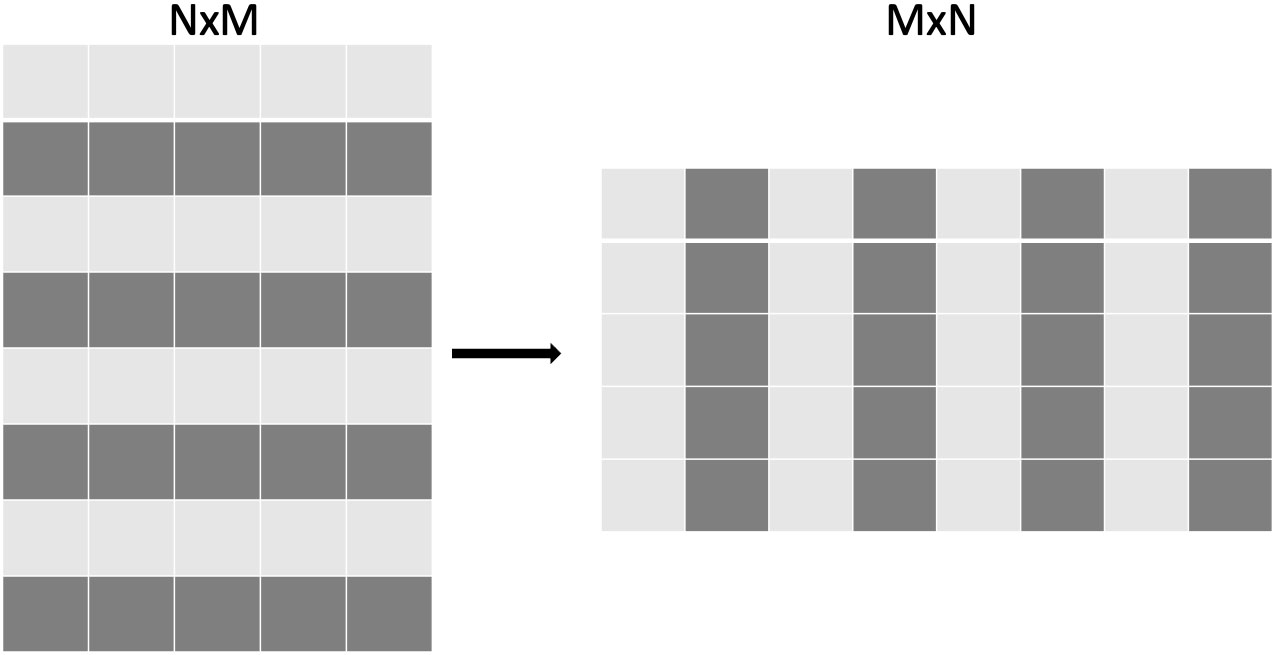
\includegraphics[width=0.8\textwidth]{fig_problem/matrix_transpose_2d.jpg}
\caption{Transpose of a (NxM) matrix to a (MxN) matrix.}\label{fig:matrix_transpose}
\end{figure}


\par
Matrix transpose~\cite{matrix_transpose} is a classic example in GPU programming where shared memory can significantly improve the performance~\cite{matrix_transpose_efficient, matrix_transpose_advanced}.
The use of shared memory reduces global memory accesses and exploits the high bandwidth and low latency of shared memory.
First as a reference we use a simple kernel which copy the data from one array to the other.
The code examples of CUDA, HIP, and SYCL are provided here \textbf{\textcolor{brown}{content/examples/exercise/non-portable-kernel-models/cuda-matrix-transpose-v0.cu}}, \textbf{\textcolor{brown}{content/examples/exercise/non-portable-kernel-models/hip-matrix-transpose-v0.cu}}, and \textbf{\textcolor{brown}{content/examples/exercise/non-portable-kernel-models/sycl-matrix-transpose-v0.cu}}, respectively in the subdirectory of this repository~\cite{gpu-programming-examples}.



\par
It should be noted that there is no calculations in these code examples.
Each thread reads one element and then writes it to another location.
By measuring the execution time of the kernel, we can compute the effective bandwidth achieve by this kernel.
Herein, we can measure the time using~\textbf{rocprof} or~\textbf{cuda/hip events}.
On a NVIDIA V100 GPU this code achieves 717 GB/s out of the theoretical peak 900 GB/s.


\par
Now we do the first iteration of the code, a~\textbf{naive transpose}.
The reading kernels in these code examples have a nice coalesced access pattern, but the writings in these code samples is very inefficient.


\par
Checking the index $in\_index$ in List~\ref{lst:09_matrix_transpose_naive_kernel_cudahip} for CUDA/HIP and List~\ref{lst:09_matrix_transpose_naive_kernel_sycl} for SYCL, we see that two adjacent threads ($threadIdx.x$, and $threadIdx.x+1$) access location in memory near each other.
However the writes are not.
Threads access data which in a strided way.
Two adjacent threads access data separated by $height$ elements.
This practically results in 32 memory operations, however due to under the hood optimizations the achieved bandwidth is 311 GB/s.


\lstinputlisting[language=c++, caption={The $transpose\_naive\_kernel$ in the~\lq\lq Matrix Transpose\rq\rq~example of CUDA/HIP.}, label={lst:09_matrix_transpose_naive_kernel_cudahip}, xleftmargin=0.05\textwidth, xrightmargin=0.05\textwidth]{code_examples/09_matrix_transpose_naive_kernel_cudahip.cpp}

\lstinputlisting[language=c++, caption={The $transposeKernel$ in the~\lq\lq Matrix Transpose\rq\rq~example of SYCL.}, label={lst:09_matrix_transpose_naive_kernel_sycl}, xleftmargin=0.05\textwidth, xrightmargin=0.05\textwidth]{code_examples/09_matrix_transpose_naive_kernel_sycl.cpp}


\par
We can improve the code efficiency by reading the data in a coalesced way, save it in the shared memory row by row and then write in the global memory column by column~\cite{matrix_transpose_efficient, matrix_transpose_advanced}.
The detailed code examples are shown in List~\ref{lst:09_matrix_transpose_sm_kernel_cudahip} for CUDA/HIP and List~\ref{lst:09_matrix_transpose_sm_kernel_sycl} for SYCL.


\lstinputlisting[language=c++, caption={The $transpose\_SM\_kernel$ in the~\lq\lq Matrix Transpose\rq\rq~example of CUDA/HIP.}, label={lst:09_matrix_transpose_sm_kernel_cudahip}, xleftmargin=0.05\textwidth, xrightmargin=0.05\textwidth]{code_examples/09_matrix_transpose_sm_kernel_cudahip.cpp}

\lstinputlisting[language=c++, caption={The $transposeKernel$ in the~\lq\lq Matrix Transpose\rq\rq~example of SYCL.}, label={lst:09_matrix_transpose_sm_kernel_sycl}, xleftmargin=0.05\textwidth, xrightmargin=0.05\textwidth]{code_examples/09_matrix_transpose_sm_kernel_sycl.cpp}


\par
In these two code examples, we define a $tile\_dim$ constant to determine the size of the shared memory tile.
The matrix transpose kernel uses a 2D grid of thread blocks, where each thread block operates on a $tile\_dim$ x $tile\_dim$ tile of the input matrix.

\par
The kernel first loads data from the global memory into the shared memory tile.
Each thread loads a single element from the input matrix into the shared memory tile.
Then, a~\textbf{\textcolor{red}{\_\_syncthreads()}} barrier ensures that all threads have finished loading data into shared memory before proceeding.


\par
Next, the kernel writes the transposed data from the shared memory tile back to the output matrix in global memory.
Each thread writes a single element from the shared memory tile to the output matrix.
By using shared memory, this optimized implementation reduces global memory accesses and exploits memory coalescence, resulting in improved performance compared to a naive transpose implementation.
This kernel achieved on NVIDIA V100 674 GB/s, which is pretty close to the bandwidth achieved by the simple copy kernel, but there is one more thing to improve.


\par
Shared memory is composed of~\textbf{banks}.
Each bank can service only one request at the time.
Bank conflicts happen when more than 1 thread in a specific warp try to access data in bank.
The bank conflicts are resolved by serializing the accesses resulting in less performance.
In the above examples when data are saved to the shared memory, each thread in the warp will save an element of the data in a different one.
Assuming that shared memory has 16 banks after writing each bank will contain one column.
At the last step when we write from the shared memory to the global memory each warp load data from the same bank.
A simple way to avoid this is by just padding the temporary array.
By padding the array, the data is slightly shifting it resulting in no bank conflicts~\cite{matrix_transpose_efficient, matrix_transpose_advanced}.
The effective bandwidth for this kernel is 697 GB/s.
The detailed code examples without bank conflicts are shown in List~\ref{lst:09_matrix_transpose_sm_nobc_kernel_cudahip} for CUDA/HIP and List~\ref{lst:09_matrix_transpose_sm_nobc_kernel_sycl} for SYCL.


\lstinputlisting[language=c++, caption={The $transpose\_SM\_nobc\_kernel$ in the~\lq\lq Matrix Transpose\rq\rq~example of CUDA/HIP.}, label={lst:09_matrix_transpose_sm_nobc_kernel_cudahip}, xleftmargin=0.05\textwidth, xrightmargin=0.05\textwidth]{code_examples/09_matrix_transpose_sm_nobc_kernel_cudahip.cpp}

\lstinputlisting[language=c++, caption={The $transposeKernel$ in the~\lq\lq Matrix Transpose\rq\rq~example of SYCL.}, label={lst:09_matrix_transpose_sm_nobc_kernel_sycl}, xleftmargin=0.05\textwidth, xrightmargin=0.05\textwidth]{code_examples/09_matrix_transpose_sm_nobc_kernel_sycl.cpp}


\par
A short summary of using the sharing memory as a cache in GPU programming.
\begin{itemize}
    \item Shared memory can significantly improve performance in operations like matrix transpose.
    \item Shared memory reduces global memory accesses and exploits the high bandwidth and low latency of shared memory.
    \item An optimized implementation utilizes shared memory, loads data coalescedly, and performs transpose operations.
    \item The optimized implementation uses a 2D grid of thread blocks and a shared memory tile size determined by a constant.
    \item The kernel loads data from global memory into the shared memory tile and uses a synchronization barrier.
    \item To avoid bank conflicts in shared memory, padding the temporary array is a simple solution.
\end{itemize}


% ---------------------------------------------------------------------- %


\subsection{Reduction}


\par
\textbf{Reduction} refers to an operation in which the elements of an array are aggregated in a single value through operations such as summing, finding the maximum or minimum, or performing logical operations.


\par
In the serial approach, the reduction is performed sequentially by iterating through the collection of values and accumulating the result step by step.
This will be enough for small sizes, but for big problems this results in significant time spent in this part of an application.
On a GPU, this approach is not feasible. Using just one thread to do this operation means the rest of the GPU is wasted.
Doing reduction in parallel is a little tricky.
In order for a thread to do work, it needs to have some partial result to use.
If we launch, for example, a kernel performing a simple vector summation, $sum[0] += a[tid]$, with $N$ threads we notice that this would result in undefined behaviour.
GPUs have mechanisms to access the memory and lock the access for other threads while one thread is doing some operations to a given data via~\textbf{atomics}, however this means that the memory access gets again to be serialized.
There is not much gain.
We note that when doing reductions the order of the iterations is not important (barring the typical non-associative behavior of floating-point operations).
Also we might have to divide the problem into several subsets and do the reduction operation for each subset separately.
On the GPUs, since the GPU threads are grouped in blocks, the size of the subset based on that.
Inside the block, threads can cooperate with each other, they can share data via the shared memory and can be synchronized as well.
All threads read the data to be reduced, but now we have significantly less partial results to deal with.
In general, the size of the block ranges from 256 to 1024 threads.
In case of very large problems, after this procedure if we are left too many partial results this step can be repeated.


\par
At the block level we still have to perform a reduction in an efficient way.
Doing it serially means that we are not using all GPU cores (roughly 97\% of the computing capacity is wasted). 
Doing it naively parallel using~\textbf{atomics}, but on the shared memory is also not a good option.
Going back to the fact the reduction operation is commutative and associative we can set each thread to~\lq\lq reduce\rq\rq~two elements of the local part of the array.
Shared memory can be used to store the partial~\lq\lq reductions\rq\rq~as shown below in the code examples of List~\ref{lst:09_reduction_cudahip} for CUDA/HIP and List~\ref{lst:09_reduction_sycl} for SYCL.


\lstinputlisting[language=c++, caption={The $reduction\_one$ kernel in the~\lq\lq Reduction\rq\rq~example of CUDA/HIP.}, label={lst:09_reduction_cudahip}, xleftmargin=0.05\textwidth, xrightmargin=0.05\textwidth]{code_examples/09_reduction_cudahip.cpp}

\lstinputlisting[language=c++, caption={The $reductionKernel$ in the~\lq\lq Reduction\rq\rq~example of SYCL.}, label={lst:09_reduction_sycl}, xleftmargin=0.05\textwidth, xrightmargin=0.05\textwidth]{code_examples/09_reduction_sycl.cpp}


\par
In the kernel we have each GPU performing thread a reduction of two elements from the local portion of the array.
If we have $tpb$ GPU threads per block, we utilize them to store $2 * tpb$ elements in the local shared memory.
To ensure synchronization until all data is available in the shared memory, we employ the~\textbf{\textcolor{red}{\_\_syncthreads()}} function.


\par
Next, we instruct each thread to~\lq\lq reduce\rq\rq~the element in the array at $threadIdx.x$ with the element at $threadIdx.x + tpb$.
As this operation saves the result back into the shared memory, we once again employ the~\textbf{\textcolor{red}{\_\_syncthreads()}} function.
By doing this, we effectively halve the number of elements to be reduced.


\par
This procedure can be repeated, but now we only utilize $tpb / 2$ threads.
Each thread is responsible for~\lq\lq reducing\rq\rq~the element in the array at $threadIdx.x$ with the element at $threadIdx.x + tpb / 2$.
After this step, we are left with $tpb / 4$ numbers to be reduced.
We continue applying this procedure until only one number remains, as shown in Fig.~\ref{fig:reduction}.


\begin{figure}[htbp]
\centering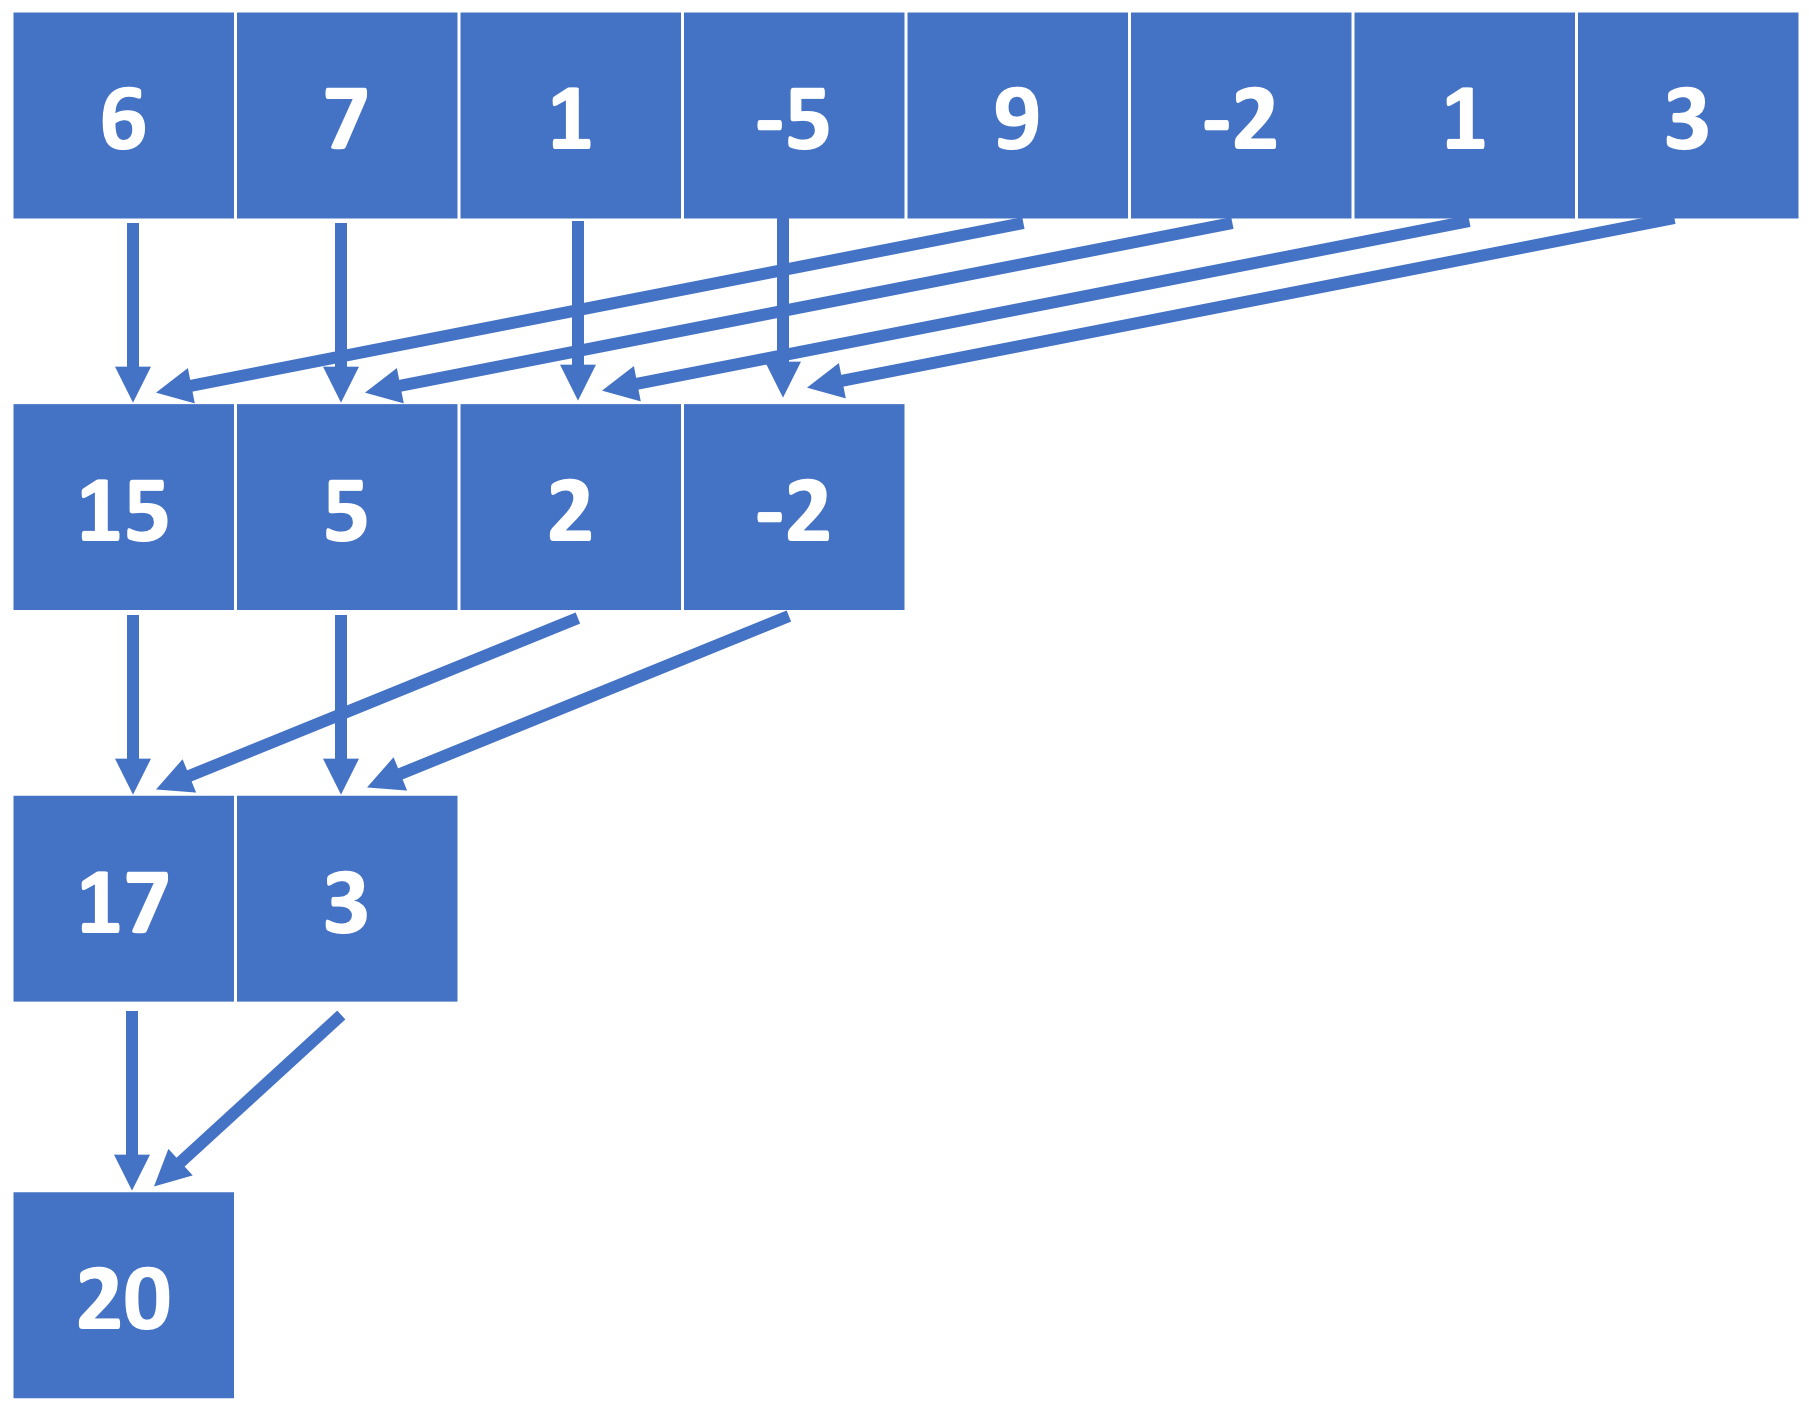
\includegraphics[width=0.6\textwidth]{fig_problem/reduction.png}
\caption{Schematic representation on the reduction algorithm with 8 GPU threads.}\label{fig:reduction}
\end{figure}


\par
At this point, we can either~\lq\lq reduce\rq\rq~the final number with a global partial result using~\textbf{atomic} read and write operations, or we can save it into an array for further processing.
For a detail analysis of how to optimize reduction operations in CUDA/HIP check the presentation~\href{https://developer.download.nvidia.com/assets/cuda/files/reduction.pdf}{Optimizing Parallel Reduction in CUDA}.


\par
Here is a short summary for reduction.
\begin{itemize}
    \item Reductions refer to aggregating elements of an array into a single value through operations like summing, finding maximum or minimum, or performing logical operations.
    \item Performing reductions sequentially in a serial approach is inefficient for large problems, while parallel reduction on GPUs offers better performance.
    \item Parallel reduction on GPUs involves dividing the problem into subsets, performing reductions within blocks of threads using shared memory, and repeatedly reducing the number of elements (two per GPU thread) until only one remains.
\end{itemize}


% ---------------------------------------------------------------------- %


\subsection{CUDA/HIP Streams}


\par
Modern GPUs can overlap independent operations.
They can do transfers between CPU and GPU and execute kernels in the same time, or they can execute kernels concurrently.
CUDA/HIP streams are independent execution units, a sequence of operations that execute in issue-order on the GPU.
The operations issue in different streams can be executed concurrently.


\par
Consider the case of~\lq\lq Vector Addition\rq\rq~discussed in previous subsection~\ref{sec:vector_addition}, which involves copying data from CPU to GPU, computations and then copying back the result to GPU, as shown in Fig.~\ref{fig:streams_timeline}.
In this way nothing can be overlapped.


\begin{figure}[htbp]
\centering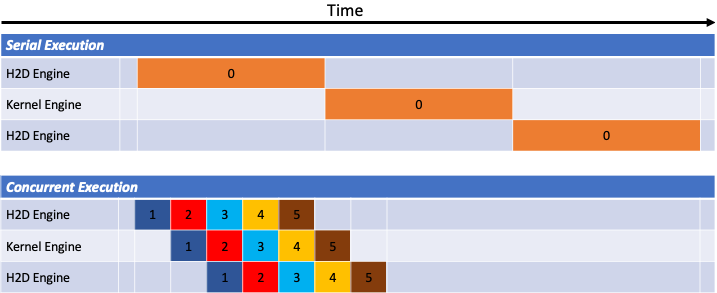
\includegraphics[width=0.8\textwidth]{fig_problem/streams_timeline.png}
\caption{The stream timelines for serial and concurrent executions in GPU programming.}\label{fig:streams_timeline}
\end{figure}


\par
We can improve the performance by dividing the problem into smaller independent parts.
Herein we consider 5 streams assuming the case where copy in one direction and computation take the same amount of time, as shown in Fig.~\ref{fig:streams_timeline}.
After the first and second stream copy data to the GPU, the GPU is practically occupied all time.
We can see that significant performance improvements can be obtained by eliminating the time in which the GPU is idle, waiting for data to arrive from the CPU.
This very useful for problems where there is often communication to the CPU because the GPU memory can not fit all the problem or the application runs in a multi-GPU set up and communication is needed often.


\par
We can apply this method to the~\lq\lq Vector Addition\rq\rq~program to expect the improvement of code examples of List~\ref{lst:09_vector_addition_stream_cuda} for CUDA and List~\ref{lst:09_vector_addition_stream_hip} for HIP.


\lstinputlisting[language=c++, caption={The application of stream method in the~\lq\lq Vector Addition\rq\rq~example of CUDA.}, label={lst:09_vector_addition_stream_cuda}, xleftmargin=0.05\textwidth, xrightmargin=0.05\textwidth]{code_examples/09_vector_addition_stream_cuda.cpp}

\lstinputlisting[language=c++, caption={The application of stream method in the~\lq\lq Vector Addition\rq\rq~example of HIP.}, label={lst:09_vector_addition_stream_hip}, xleftmargin=0.05\textwidth, xrightmargin=0.05\textwidth]{code_examples/09_vector_addition_stream_hip.cpp}


\par
It is clearly shown in these code examples that instead of having one copy to GPU, one execution of the kernel and one copy back, we now have several of these calls independent of each other.
Note that even when streams are not explicitly used, it is possible to launch all the GPU operations asynchronous and overlap CPU operations (such I/O) and GPU operations.
In order to learn more about how to improve performance using CUDA/HIP streams, one should check the NVIDIA blog\href{https://developer.nvidia.com/blog/how-overlap-data-transfers-cuda-cc/}{How to Overlap Data Transfers in CUDA C/C++}.


\par
Here is a short summary for CUDA/HIP streams.
\begin{itemize}
    \item CUDA/HIP streams are independent execution contexts on the GPU that allow for concurrent execution of operations issued in different streams.
    \item Using streams can improve GPU performance by overlapping operations such as data transfers between CPU and GPU and kernel executions.
    \item By dividing a problem into smaller independent parts and utilizing multiple streams, the GPU can avoid idle time, resulting in significant performance improvements, especially for problems with frequent CPU communication or multi-GPU setups.
\end{itemize}


% ---------------------------------------------------------------------- %


\subsection{Pros and cons of native programming models}


\par
There are advantages and limitations to native GPU programming models of CUDA and HIP:
\begin{itemize}
    \item~\textbf{CUDA Pros}:
    \begin{itemize}
        \item Performance Boost: CUDA is designed for NVIDIA GPUs and delivers excellent performance.
        \item Wide Adoption: CUDA is popular, with many resources and tools available.
        \item Mature Ecosystem: NVIDIA provides comprehensive libraries and tools for CUDA programming.
    \end{itemize}
    \item~\textbf{HIP Pros}:
    \begin{itemize}
        \item Portability: HIP is portable across different GPU architectures.
        \item Open Standards: HIP is based on open standards, making it more accessible.
        \item Growing Community: The HIP community is growing, providing more resources and support.
    \end{itemize}
    \item~\textbf{Cons}:
    \begin{itemize}
        \item Exclusive for GPUs
        \item Vendor Lock-in: CUDA is exclusive to NVIDIA GPUs, limiting compatibility.
        \item Learning Curve: Both CUDA and HIP require learning GPU programming concepts.
        \item Limited Hardware Support: HIP may face limitations on older or less common GPUs.
    \end{itemize}
\end{itemize}

